% !TEX root = ../../main.tex
\section{Вибірка та її первинний аналіз}
\subsection{Поняття вибірки}
Математична статистика вивчає випадкові величини за певними дослідними даними, які отримано в ході експерименту.
Коротко кажучи, методами математичної статистики можна оцінювати (але не визначати точно) числові характеристики 
та розподіл деякої випадкової величини,
якщо відомо деякий набір значень, яких ця величина набула в ході досліду. При цьому, зазвичай, апріорних відомостей про
цю випадкову величину майже немає.
\begin{definition}\index{генеральна сукупність}
    \emph{Генеральною сукупністю (ГС)} називають як випадкову величину $\xi$, що досліджується, так і множину всіх її можливих значень.
\end{definition}
\begin{definition}\index{вибірка!випадкова}\index{вибірка!реалізація вибірки}\index{вибірка!вибірковий простір}
    \emph{Випадковою вибіркою обсягу $n$} називається випадковий вектор $\left( \xi_1, ..., \xi_n\right)$, координати якого є однаково
    розподіленими, як ГС, і незалежними в сукупності. Підмножина $G\subseteq \mathbb{R}^n$, що складається з усіх можливих значень визначеної вище
    випадкової вибірки, називається $\emph{вибірковим простором}$, а вектори $\vec{x} \in G$ --- \emph{реалізаціями вибірки}.
    \emph{Конкретною реалізацією вибірки} інколи називають саме ту реалізацію, з якою працюють після проведення експерименту.
\end{definition}
\begin{example}
    Нехай $\xi \sim \mathrm{Bin}(N, p)$, $N = 3$. В цьому випадку $G = \left\{0, 1, 2, 3\right\}^{\times n}$ --- множина
    $n$-вимірних векторів, всі координати яких набувають лише значень $0$, $1$, $2$ та $3$.
\end{example}
\begin{remark}\index{вибірка!репрезентативна}\index{вибірка!стратифікована}
    В прикладній статистиці зазвичай не користуються таким різноманітним набором означень. Там під вибіркою розуміють як і будь-які 
    отримані внаслідок експерименту спостереження, так і процес їх отримання. Варто навести два означення, які, хоч і не будуть застосовуватися далі
    в курсі, але зустрічаються в прикладній статистиці. \emph{Репрезентативна вибірка} --- така, яка має всі властивості генеральної сукупності. Інакше кажучи, всі можливі значення 
    (або проміжки значень) ГС мають однакову ймовірність потрапити до конкретної реалізації вибірки.
    \emph{Стратифікована вибірка} --- така, що гарантує збереження пропорцій, наявних у ГС.
    Наприклад, якщо мова йде про результати якогось опитування, то репрезентативна вибірка має містити результати всіх категорій населення, а 
    стратифікована ще й має містити їх в тих пропорціях, які ці категорії складають в усьому населенні країни.
    На практиці поняття репрезентативної та стратифікованої вибірки залежать від ГС, структуру та природу якої дослідник попередньо вивчає,
    та від мети самого дослідження: наприклад, населення всієї країни може грати роль ГС у багатьох статистичних дослідженнях, 
    але його поділ на категорії може відрізнятися.
\end{remark}
\subsection{Розподіл випадкової вибірки}
Нехай $\vec{\xi} = \left( \xi_1, ..., \xi_n\right)$ --- випадкова вибірка, а $F_{\xi}(x)$ --- функція розподілу ГС. Тоді для 
$\vec{x} \in \mathbb{R}^n$ визначено функцію розподілу 
$F_{\vec{\xi}}(\vec{x}) = \P\left\{\xi_1 < x_1, ..., \xi_n < x_n \right\} = \prod\limits_{k=1}^n F_{\xi}(x_k)$. Для досліджень вибірок, однак,
зручно користуватися іншою функцією.
\begin{definition}\index{функція правдоподібності}
    \emph{Функцією правдоподібності} випадкової вибірки обсягу $n$ з ГС $\xi$ називається 
    \begin{gather}
        \mathcal{L}(\vec{x}) = \prod\limits_{k=1}^n \P\left\{ \xi = x_k\right\}, \text{ якщо } \xi \text{ --- ДВВ} \\
        \mathcal{L}(\vec{x}) = \prod\limits_{k=1}^n f_{\xi}(x_k) \text{ якщо } \xi \text{ --- НВВ}
    \end{gather}
\end{definition}
Часто аргументами функції правдоподібності вважають параметри закону розподілу ГС. В такому випадку при фіксованому значенні
$\vec{x}$ ця функція фактично показує, як в залежності від параметрів розподілу змінюється ймовірність отримати саме таку реалізацію
вибірки --- $\left(x_1, ..., x_n \right)$.
Отримаємо функції правдоподібності для основних законів розподілу. В подальшому будуть більш корисними не самі функції правдоподібності,
а їх логарифми.
\begin{enumerate}
    \item $\xi \sim \mathrm{Bin}(N,p)$ --- біноміальний розподіл, $\forall \; k \in \mathbb{N} \; x_k \in \left\{0, 1, ..., N \right\}$:
    \begin{gather*}
        \mathcal{L}_{\mathrm{Bin}}(\vec{x}, N, p) = \prod\limits_{k=1}^n C_N^{x_k} p^{x_k} (1-p)^{N - x_k} = 
        \prod\limits_{k=1}^n C_N^{x_k} \cdot p^{\sum_{k=1}^n x_k} \cdot (1-p)^{N\cdot n - \sum_{k=1}^n x_k} \\
        \ln \mathcal{L}_{\mathrm{Bin}}(\vec{x}, N, p) = \sum\limits_{k=1}^n \ln C_N^{x_k} + \ln p \cdot \sum\limits_{k=1}^n x_k + 
        \ln{(1-p)} \cdot\left( N\cdot n - \sum\limits_{k=1}^n x_k\right)
    \end{gather*}
    \item $\xi \sim \mathrm{Geom}(p)$ --- геометричний розподіл, $\forall \; k \in \mathbb{N} \; x_k \in \left\{1, 2, 3, ...\right\}$. 
    \begin{gather*}
        \mathcal{L}_{\mathrm{Geom}}(\vec{x}, p) = \prod\limits_{k=1}^n p (1-p)^{x_k - 1} = p^n \cdot (1-p)^{\sum_{k=1}^n x_k - n} \\
        \ln \mathcal{L}_{\mathrm{Geom}}(\vec{x}, p) = n \ln p + \ln{(1-p)} \cdot\left(\sum\limits_{k=1}^n x_k - n\right)
    \end{gather*}
    \item $\xi \sim \mathrm{Pas}(a)$ --- розподіл Паскаля, $\forall \; k \in \mathbb{N} \; x_k \in \left\{0, 1, 2, 3, ...\right\}$. 
    \begin{gather*}
        \mathcal{L}_{\mathrm{Pas}}(\vec{x}, a) = \prod\limits_{k=1}^n \frac{a^{x_k}}{(1+a)^{x_k + 1}} = 
        \frac{a^{\sum_{k=1}^n x_k}}{(1+a)^{n + \sum_{k=1}^n x_k}} \\
        \ln \mathcal{L}_{\mathrm{Pas}}(\vec{x}, a) = \ln a \cdot \sum\limits_{k=1}^n x_k - \ln{(1+a)} \cdot \left(n+ \sum\limits_{k=1}^n x_k\right) 
    \end{gather*}
    \item $\xi \sim \mathrm{Poiss}(a)$ --- розподіл Пуассона, $\forall \; k \in \mathbb{N} \; x_k \in \left\{0, 1, 2, 3, ...\right\}$. 
    \begin{gather*}
        \mathcal{L}_{\mathrm{Poiss}}(\vec{x}, a) = \prod\limits_{k=1}^n \frac{a^{x_k}}{(x_k)!} e^{-a} = e^{-na} \cdot \frac{a^{\sum\limits_{k=1}^n x_k}}{\prod\limits_{k=1}^n x_k !} \\
        \ln \mathcal{L}_{\mathrm{Poiss}}(\vec{x}, a) = -n a + \ln a \cdot \sum\limits_{k=1}^n x_k - \sum\limits_{k=1}^n \ln{x_k!}
    \end{gather*}
    \item $\xi \sim \mathrm{U}\left< a; b\right>$ --- рівномірний розподіл, $\forall \; k \in \mathbb{N} \; x_k \in \left< a; b\right>$:
    \begin{gather*}
        \mathcal{L}_{\mathrm{U}}(\vec{x}, a, b) = \prod\limits_{k=1}^n \frac{1}{b-a} = \frac{1}{(b-a)^n} \\
        \ln\mathcal{L}_{\mathrm{U}}(\vec{x}, a, b) = -n \ln{(b-a)}
    \end{gather*} 
    \item $\xi \sim \mathrm{Exp}(\lambda, b)$ --- експоненційний розподіл зі зсувом, $\forall \; k \in \mathbb{N} \; x_k \geq b$:
    \begin{gather*}
        \mathcal{L}_{\mathrm{Exp}}(\vec{x}, \lambda, b) = \prod\limits_{k=1}^n \lambda e^{-\lambda (x_k-b)} = \lambda^n e^{-\lambda\left(\sum\limits_{k=1}^n x_k - n b\right)} \\
        \ln \mathcal{L}_{\mathrm{Exp}}(\vec{x}, \lambda, b) = n \ln \lambda - \lambda\left(\sum\limits_{k=1}^n x_k - n b\right)
    \end{gather*}
    \item $\xi \sim \mathrm{N}(a, \sigma^2)$ --- нормальний розподіл, $\forall \; k \in \mathbb{N} \; x_k \in \mathbb{R}$:
    \begin{gather*}
        \mathcal{L}_{\mathrm{N}}(\vec{x}, a, \sigma) = \prod\limits_{k=1}^n \frac{1}{\sqrt{2\pi}\sigma} \exp\left\{-\frac{(x_k - a)^2}{2\sigma^2}\right\} =
        \frac{1}{(2\pi)^{\frac{n}{2}} \sigma^n} \cdot \exp\left\{-\frac{1}{2\sigma^2}\sum\limits_{k=1}^n (x_k - a)^2\right\}\\
        \ln \mathcal{L}_{\mathrm{N}}(\vec{x}, a, \sigma) = -\frac{n}{2}\ln{2\pi} - n \ln{\sigma} - \frac{1}{2\sigma^2}\sum\limits_{k=1}^n (x_k - a)^2
    \end{gather*}
\end{enumerate}

\subsection{Дискретний варіаційний ряд}
Нехай $\left(x_1, ... ,x_n\right)$ --- конкретна реалізація вибірки, що містить небагато (порівняно з обсягом вибірки) унікальних значень,
які називаються \emph{варіантами} та позначаються $x_i^*$.
\begin{definition}\index{варіаційний ряд!дискретний}
    \emph{Дискретним варіаційним рядом (ДВР)} називається таблиця вигляду
    \begin{center}
    \begin{tabular}{|c|c|c|c|c|}
        \hline
        варіанти & $x_1^*$ & $x_2^*$ & $...$ & $x_r^*$ \\
        \hline
        частоти $n_i$ & $n_1$ & $n_2$ & $...$ & $n_r$ \\
        \hline
        частості $\omega_i $& $\frac{n_1}{n}$ & $\frac{n_2}{n}$ & $...$ & $\frac{n_r}{n}$ \\
        \hline
    \end{tabular}
    \end{center}
    Тут $x_1^* < x_2^* < ... < x_r^*$, частоти --- кількість входжень відповідної варіанти до реалізації вибірки, $\sum\limits_{i=1}^r n_i = n$, $\sum\limits_{i=1}^r \omega_i = 1$.
    Частості ще називають відносними частотами.
    Іноді до ДВР вносять накопичені частості $\omega_i^{\text{нак}}$: $\omega_1^{\text{нак}} = \frac{n_1}{n} = \omega_1$, $\omega_2^{\text{нак}} = \frac{n_1+n_2}{n}$ і т.д., $w_r^{\text{нак}} = 1$.
\end{definition}
\index{полігон!відносних частот}
Геометричною інтерпретацію ДВР є \emph{полігон відносних частот} з вершинами $\left( x_i^*, \omega_i\right)$:
\begin{center}
    \begin{tikzpicture}
        \pgfmathsetmacro{\s}{0.6};
        \pgfmathsetmacro{\t}{1.5};
        \draw [->] (0,0) -- (5*\t,0);
        \draw [->] (0,0) -- (0,6*\s);
        \draw [fill] (1*\t, 0) circle [radius = 0.05];
        \node [below] at (1*\t, 0) {$x_1^*$};
        \node [below] at (2*\t, 0) {$x_2^*$};
        \node [below] at (3*\t, 0) {$x_3^*$};
        \node [below] at (3.75*\t, 0) {$...$};
        \node [below] at (4.5*\t, 0) {$x_r^*$};
        \node [left] at (0, 1*\s) {$\omega_1$};
        \node [left] at (0, 2*\s) {$\omega_3$};
        \node [left] at (0, 3*\s) {$\omega_2$};
        \node [left] at (0, 3.75*\s) {$...$};
        \node [left] at (0, 4.5*\s) {$\omega_r$};
        \draw [fill] (2*\t, 0) circle [radius = 0.05];
        \draw [fill] (3*\t, 0) circle [radius = 0.05];
        \draw [fill] (4.5*\t, 0) circle [radius = 0.05];
        \draw [fill] (0, 1*\s) circle [radius = 0.05];
        \draw [fill] (0, 2*\s) circle [radius = 0.05];
        \draw [fill] (0, 3*\s) circle [radius = 0.05];
        \draw [fill] (0, 4.5*\s) circle [radius = 0.05];
        \draw [fill] (0, 5.5*\s) circle [radius = 0.05];
        \node [left] at (0, 5.5*\s) {$1$};
        \node [right] at (5*\t, 0) {$x$};
        \node [above] at (0, 6*\s) {$\omega$};
        \draw [dashed] (0, 5.5*\s) -- (5*\t, 5.5*\s);
        \draw [fill] (1*\t, 1*\s) circle [radius = 0.05];
        \draw [fill] (2*\t, 3*\s) circle [radius = 0.05];
        \draw [fill] (3*\t, 2*\s) circle [radius = 0.05];
        \draw [fill] (4.5*\t, 4.5*\s) circle [radius = 0.05];
        \draw (1*\t, 1*\s) -- (2*\t, 3*\s) -- (3*\t, 2*\s);
        \draw [dashed] (3*\t, 2*\s) -- (4.5*\t, 4.5*\s);
    \end{tikzpicture}
\end{center}
Якщо в конкретній реалізації вибірки унікальних значень досить мало, то можна висунути припущення, що ГС має дискретний розподіл.
В такому випадку вигляд полігону частостей може допомогти висунути припущення про закон розподілу. 
Перевірку таких припущень буде розглянуто пізніше.

\subsection{Інтервальний варіаційний ряд}
Нехай $\left(x_1, ... ,x_n\right)$ --- конкретна реалізація вибірки, майже всі значення якої є унікальними. В такому випадку
дискретний варіаційний ряд будувати недоцільно.
\begin{definition}\index{варіаційний ряд!інтервальний}
    \emph{Інтервальний варіаційним рядом (ІВР)} називається таблиця вигляду
    \begin{center}
        \begin{tabular}{|c|c|c|c|c|}
            \hline
            інтервал $\Delta_i$ & $[x_{\min}; t_1)$ & $[t_1; t_2)$ & $...$ & $[t_r, x_{\max}]$ \\
            \hline
            частоти $n_i$ & $n_1$ & $n_2$ & $...$ & $n_{r+1}$ \\
            \hline
            частості $\omega_i$ & $\frac{n_1}{n}$ & $\frac{n_2}{n}$ & $...$ & $\frac{n_{r+1}}{n}$ \\
            \hline
        \end{tabular}
        \end{center}
        Тут $x_{\min}$ та $x_{\max}$ --- мінімальне та максимальне значення цієї реалізації вибірки ($R = x_{\max} - x_{\min}$ називається \emph{розмахом вибірки}), а $t_i$ --- деякі точки всередині відрізка 
        $[x_{\min}; x_{\max}]$. Немає універсальної рекомендації для вибору значень та кількості $t_i$. На практиці часто користуються \emph{правилом Стерджеса}:
        відрізок $[x_{\min}; x_{\max}]$ ділиться на $k = 1 + \left[ 3.322 \lg n\right]$ інтервалів рівної довжини. Іноді можна зустріти формулу
        $k = 1 + \left[\log_2 n\right]$, яка еквівалентна попередній, оскільки $\log_2 n = \log_2 10 \cdot \lg n \approx 3.322 \lg n$.
\end{definition}
\index{гістограма}
Геометричною інтерпретацію ІВР є \emph{гістограма}, що складається з прямокутників, що побудовані на $\Delta_i$ та мають висоти $h_i = \frac{\omega_i}{d_i}$, де $d_i$ --- довжина $\Delta_i$:
\begin{center}
    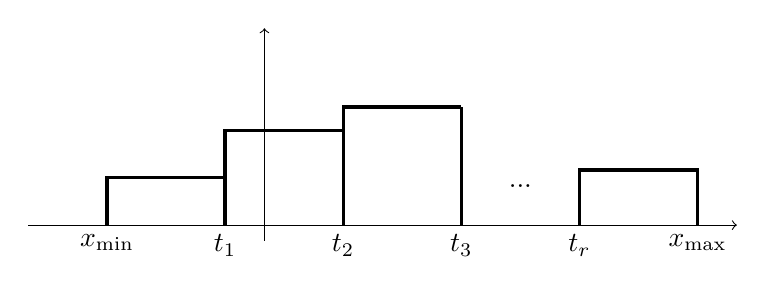
\begin{tikzpicture}
        \draw [->] (-3,0) -- (6,0);
        \draw [->] (0,-0.2) -- (0,2.5);
        \draw [very thick] (-2, 0) -- (-2, 0.6) -- (-0.5, 0.6);
        \draw [very thick] (-0.5, 0) -- (-0.5, 1.2) -- (1, 1.2);
        \draw [very thick] (1, 0) -- (1, 1.5) -- (2.5, 1.5);
        \draw [very thick] (2.5, 0) -- (2.5, 1.5);
        \node at (3.25, 0.5) {$...$};
        \draw [very thick] (4, 0) -- (4, 0.7) -- (5.5, 0.7) -- (5.5, 0);
        \node [below] at (-2, 0) {$x_{\min}$};
        \node [below] at (-0.5, 0) {$t_1$};
        \node [below] at (1, 0) {$t_2$};
        \node [below] at (2.5, 0) {$t_3$};
        \node [below] at (4, 0) {$t_r$};
        \node [below] at (5.5, 0) {$x_{\max}$};
    \end{tikzpicture}
\end{center}

Якщо в конкретній реалізації вибірки багато унікальних значень, то можна висунути припущення, що ГС має неперервний розподіл.
В такому випадку вигляд гістограми може допомогти висунути припущення про закон розподілу. Нескладно помітити, що сумарна площа прямокутників у гістограмі
$\sum\limits_{i=1}^{r+1} d_i \cdot \frac{\omega_i}{d_i} = 1$, тому в деякому сенсі гістограма є аналогом графіка щільності розподілу. Зауважимо, що в разі
невдало вибраної кількості інтервалів (забагато чи замало) гістограма буде погано відображати характер отриманої реалізації вибірки.

\subsection{Емпірична функція розподілу}
\index{функція розподілу!емпірична}
Користуючись варіаційними рядами, для конкретної реалізації вибірки можна побудувати \emph{емпіричну функцію розподілу} $F_n^*(x)$, яка визначається наступним чином:
\begin{center}
    \begin{tabular}{c c}
        $F_n^*(x) = \begin{cases}
            0, & x \leq x_1^* \\
            \omega_1^{\text{нак}} = \frac{n_1}{n}, & x_1^* < x \leq x_2^* \\
            \omega_2^{\text{нак}} = \frac{n_1+n_2}{n}, & x_2^* < x \leq x_3^* \\
            ... \\
            1, & x > x_r^*
        \end{cases}$ &
        $F_n^*(x) = \begin{cases}
            0, & x \leq x_{\min} \\
            \omega_1^{\text{нак}} = \frac{n_1}{n}, & x_{\min} < x \leq t_1 \\
            \omega_2^{\text{нак}} = \frac{n_1+n_2}{n}, & t_1 < x \leq t_2 \\
            ... \\
            1, & x > t_r
        \end{cases}$ \\
        для ДВР & для ІВР 
    \end{tabular}
\end{center}

Існує й інше означення, більш коректне з теоретичної точки зору та універсальне.
\begin{definition}
    \emph{Емпіричною функцією розподілу (ЕФР)}, побудованою за випадковою вибіркою $\vec{\xi} = \left( \xi_1, ..., \xi_n\right)$, називається випадкова функція 
    $F_n^* : \mathbb{R}\times \Omega \to [0; 1]$, що задана як
    \begin{gather}
        F_n^*(x) = \frac{1}{n} \sum\limits_{k=1}^n \mathds{1}{\left\{ \xi_k < x\right\}}
    \end{gather}
    Тут $\mathds{1}{\left\{ \xi_k < x\right\}}$ --- індикатор події $\left\{ \xi_k < x\right\}$, що дорівнює $1$ з ймовірністю $p = \P\left\{ \xi_k < x\right\} = F_{\xi}(x)$ та
    $0$ з ймовірністю $1-p$.       
\end{definition}
\begin{remark}
    Поняття випадкової функції тут, по суті, не є новим --- це випадкова величина, що залежить від дійсного параметру (в цьому випадку $x$).
\end{remark}
Таким чином, означення ЕФР, наведені спочатку, є значеннями цієї випадкової функції при фіксованих значеннях $\vec{\xi}$.
Наступна теорема ілюструє важливість означення ЕФР саме як випадкової функції.
\begin{theorem*}[теорема Глівенко-Кантеллі]\index{теорема!Глівенко-Кантеллі}
    $$
    \forall \; x\in\mathbb{R}: F_n^* (x) \overset{\mathrm{P1}}{\longrightarrow} F_{\xi}(x), \; n\to\infty
    $$
\end{theorem*}
\begin{proof}
    Для всіх $k \in \mathbb{N} \text{ та } x \in\mathbb{R} :  \E\left(\mathds{1}{\left\{ \xi_k < x\right\}}\right) = F_{\xi}(x)$, причому при будь-якому $x \in \mathbb{R}$ ці індикатори
    є незалежними випадковими величинами. Тому згідно посиленого закону великих чисел отримуємо бажану збіжність з ймовірністю 1 до $F_{\xi}(x)$.
\end{proof}
\begin{exercise}
    Довести теорему Глівенко-Кантеллі безпосередньо, скориставшись достатньою ознакою збіжності з ймовірністю 1:
    якщо для будь-якого $\varepsilon >0$ ряд
    $\sum\limits_{n=1}^{\infty} \P\left\{\left| \xi_n - \xi\right| > \varepsilon\right\}$ збігається, то 
    $\xi_n \overset{\mathrm{P1}}{\longrightarrow} \xi, n \to \infty$. Підказка: треба оцінити 
    $\P\left\{\left|F_n^* (x) - F_{\xi}(x)\right| > \varepsilon\right\}$ членами збіжного ряду.
\end{exercise}

\subsection{Вибіркові характеристики ГС}
\begin{definition}\index{статистика}
    \emph{Статистикою} називається випадкова величина, що є функцією від випадкової вибірки $h = h( \vec{\xi})$.
\end{definition}
Розглянемо деякі статистики, які в деякому сенсі є аналогами числових характеристик для ГС.
Пізніше буде розглянуто застосування цих статистик для висування та перевірки припущень про розподіл ГС.
\begin{enumerate}
    \item \emph{Емпіричні початкові моменти $k$-того порядку} \index{момент!початковий!емпіричний}
    $\E^* \xi^k = \frac{1}{n}\sum\limits_{i=1}^n \xi_i^k$. Значення на конкретній реалізації вибірки позначається як
    $(\E^* \xi^k)_{\text{зн}} = \frac{1}{n}\sum\limits_{i=1}^n x_i^k$. Окремим випадком емпіричних початкових моментів
    є \emph{вибіркове середнє} \index{математичне сподівання!вибіркове} $\overline{\xi} = \frac{1}{n}\sum\limits_{i=1}^n \xi_i$, значення якого позначається як
    $\overline{x} = \frac{1}{n}\sum\limits_{i=1}^n x_i$. Після складання варіаційного ряду можна записати значення
    вибіркового середнього як $$\overline{x} = \begin{cases}
        \frac{1}{n} \sum\limits_{i=1}^r x_i^* n_i & \text{ для ДВР} \\
        \frac{1}{n} \sum\limits_{i=1}^{r+1} x_i^* n_i & \text{ для ІВР}
    \end{cases}$$
    У випадку ІВР за $x_i^*$ береться довільний представник $i$-того інтервалу.
    \item \emph{Емпіричні центральні моменти $k$-того порядку} \index{момент!центральний!емпіричний}
    $\E^* \mathring{\xi}^k$ можуть вводитися двома способами: як 
    $\frac{1}{n}\sum\limits_{i=1}^n \left(\xi_i - \E\xi \right)^k$, якщо $\E\xi$ відоме, або як 
    $\frac{1}{n}\sum\limits_{i=1}^n \left(\xi_i - \overline{\xi} \right)^k$, якщо $\E\xi$ невідоме.
    Окремим випадком є \emph{вибіркова дисперсія} \index{дисперсія!вибіркова} $\D^* \xi$ при $k=2$. Її значення позначається як 
    $(\D^* \xi)_{\text{зн}} = \frac{1}{n}\sum\limits_{i=1}^n \left(x_i - \E\xi \right)^2$ або 
    $\frac{1}{n}\sum\limits_{i=1}^n \left(x_i - \overline{x} \right)^2$.
    \item \emph{Вибіркова мода} \index{мода!вибіркова}$\mathrm{Mo}^* \xi$ у випадку побудови ДВР визначається як варіанта з найбільшою частістю, а у випадку
    ІВР --- за формулою $(\mathrm{Mo}^* \xi)_{\text{зн}} = y_i + h_i \cdot \frac{n_i - n_{i-1}}{(n_i - n_{i-1}) + (n_i - n_{i+1})}$, де $y_i$ --- початок інтервалу,
    якому відповідає найбільша частість (модальний інтервал), а $h_i$ --- довжина цього інтервалу, а $n_i$ --- частоти.
    \item \emph{Вибіркова медіана} \index{медіана!вибіркова} $\mathrm{Me}^* \xi$ у випадку побудови ДВР визначається як середня за розташуванням варіанта (або середнє арифметичне 
    таких варіант, якщо їх парна кількість), а у випадку ІВР --- за формулою 
    $(\mathrm{Me}^* \xi)_{\text{зн}} = y_i + \frac{h_i}{n_i} \cdot \left(\frac{n}{2} - \sum\limits_{k=1}^{i-1} n_k \right)$, де 
    $y_i$ --- початок інтервалу, на якому накопичена частість перевищила $0.5$ (медіанний інтервал), $h_i$ --- його довжина,
    $n_i$ --- частоти.
    \item \emph{Вибіркова асиметрія та вибірковий ексцес} \index{асиметрія!вибіркова}\index{ексцес!вибірковий} визначаються як 
    $\mathrm{As}^* \xi = \frac{\frac{1}{n}\sum\limits_{i=1}^n \left(\xi_i - \overline{\xi} \right)^3}{(\D^*\xi)^{3/2}}$ та
    $\mathrm{Ex}^* \xi = \frac{\frac{1}{n}\sum\limits_{i=1}^n \left(\xi_i - \overline{\xi} \right)^4}{(\D^*\xi)^{2}} - 3$ з заміною
    $\overline{\xi}$ на $\E\xi$, якщо воно відоме.
\end{enumerate}

\subsection{Діаграми розмаху}
\index{діаграма розмаху}
Розглянемо спосіб візуалізації реалізацій вибірки, який часто застосовується на практиці через свою інформативність.
\begin{center}
    \begin{tikzpicture}
        \draw [thick, dashed] (-6, 0) -- (-2, 0);
        \draw [thick, dashed] (3, 0) -- (6, 0);
        \draw [thick] (-6, -0.5) -- (-6, 0.5);
        \draw [thick] (6, -0.5) -- (6, 0.5);
        \draw [fill] (-6.2, 0) circle [radius = 0.07];
        \draw [fill] (-6.6, 0) circle [radius = 0.07];
        \draw [fill] (6.3, 0) circle [radius = 0.07];
        \draw [fill] (7.5, 0) circle [radius = 0.07];
        \draw [thick] (-2, -1) -- (-2, 1) -- (3, 1) -- (3, -1) -- (-2, -1);
        \draw [ultra thick] (1, -1) -- (1, 1);
    \end{tikzpicture}
\end{center}
Для спрощення опису в межах цього пункту називатимемо конкретну реалізацію вибірки просто вибіркою.
Горизонтальна вісь такої діаграми відповідає діапазону значень вибірки. Межами прямокутника (через який цю діаграму ще називають
\emph{коробковою}) є \emph{1 та 3 квартилі вибірки}, що позначаються $Q_1$ та $Q_3$ --- це медіани першої та другої половини відсортованої вибірки (які у випадку
непарного обсягу розділяються медіаною вибірки).
Різниця ${IQR} = Q_3 - Q_1$ (довжина прямокутника) називається \emph{міжквартильним розмахом}. Відрізок всередині прямокутника позначає положення \emph{медіани}.
Вертикальні відрізки за межами прямокутника (які ще називають \emph{вусами}) позначають <<майже мінімум і максимум>>: зазвичай вони знаходяться
в положеннях $Q_1 - 1.5\cdot{IQR}$ та $Q_3 + 1.5\cdot{IQR}$. Усі значення, що менше <<мінімуму>> та більше <<максимуму>>, називаються \emph{викидами} та 
позначаються окремими точками. На практиці для подальшої обробки викиди прибирають з вибірки, оскільки такі значення можуть з'являтися через помилки вимірювань.

\begin{example}
    Побудувати діаграму розмаху для вибірки ($n = 20$):
    \begin{center}
        \begin{tabular}{c c c c c c c c c c}
            $-0.005$ & $-0.111$ & $0.384$ & $0.413$ & $-0.152$ & $-0.453$ & $-0.273$ & $0.366$ & $0.331$ & $1.147$ \\
            $0.425$ & $0.166$ & $0.512$ & $0.789$ & $0.686$ & $-0.205$ & $0.175$ & $0.092$ & $1.72$ & $1.43$
            \end{tabular}
    \end{center}
    Після сортування за зростанням отримаємо 
    \begin{center}
        \begin{tabular}{c c c c c c c c c c}
            $-0.453$ & $-0.273$ & $-0.205$ & $-0.152$ & $-0.111$ & $-0.005$ & $0.092$ & $0.166$ & $0.175$ & $0.331$ \\
            $0.366$ & $0.384$ & $0.413$ & $0.425$ & $0.512$ & $0.686$ & $0.789$ & $1.147$ & $1.43$ & $1.72$
            \end{tabular}
    \end{center}
    Медіана дорівнює $\frac{0.331+0.366}{2} = 0.3385$, а квартилі --- $Q_1 = \frac{-0.111 - 0.005}{2} = -0.058$,
    $Q_3 = \frac{0.512 + 0.686}{2} = 0.599$. Міжквартильний розмах ${IQR} = Q_3 - Q_1 = 0.657$, далі обчислимо
    $Q_1 - 1.5\cdot{IQR} = -1.0435$ та $Q_3 + 1.5\cdot{IQR} = 1.5845$. Отже, значення 1.72 є викидом.
    Нарешті, побудуємо діаграму розмаху:
    \begin{center}
        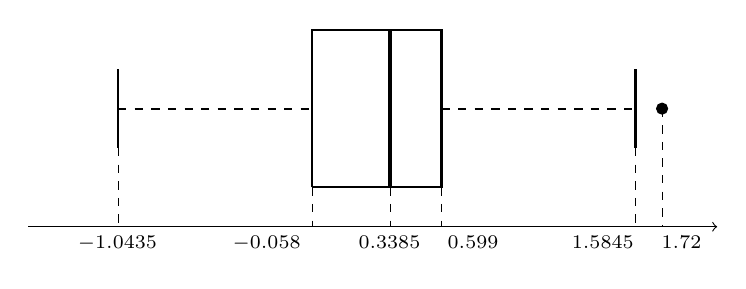
\begin{tikzpicture}
            \pgfmathsetmacro{\xs}{2.5};
            \pgfmathsetmacro{\qo}{-0.058};
            \pgfmathsetmacro{\qt}{0.599};
            \pgfmathsetmacro{\me}{0.3385};
            \pgfmathsetmacro{\min}{-1.0435};
            \pgfmathsetmacro{\max}{1.5845};
            \pgfmathsetmacro{\out}{1.72};
            \draw [->] (-1.5*\xs, -1.5) -- (2*\xs, -1.5);
            \draw [thick, dashed] (\min*\xs, 0) -- (\qo*\xs, 0);
            \draw [thick, dashed] (\qt*\xs, 0) -- (\max*\xs, 0);
            \draw [thick] (\min*\xs, -0.5) -- (\min*\xs, 0.5);
            \draw [thick] (\max*\xs, -0.5) -- (\max*\xs, 0.5);
            \draw [fill] (\out*\xs, 0) circle [radius = 0.07];
            \draw [thick] (\qo*\xs, -1) -- (\qo*\xs, 1) -- (\qt*\xs, 1) -- (\qt*\xs, -1) -- (\qo*\xs, -1);
            \draw [ultra thick] (\me*\xs, -1) -- (\me*\xs, 1);
            \draw [dashed] (\me*\xs, -1) -- (\me*\xs, -1.5);
            \draw [dashed] (\qo*\xs, -1) -- (\qo*\xs, -1.5);
            \draw [dashed] (\qt*\xs, -1) -- (\qt*\xs, -1.5);
            \draw [dashed] (\min*\xs, -0.5) -- (\min*\xs, -1.5);
            \draw [dashed] (\max*\xs, -0.5) -- (\max*\xs, -1.5);
            \draw [dashed] (\out*\xs, 0) -- (\out*\xs, -1.5);
            \node [below] at (\me*\xs, -1.5) {$_{\me}$};
            \node [below left] at (\qo*\xs*1.03, -1.5) {$_{\qo}$};
            \node [below right] at (\qt*\xs*0.97, -1.5) {$_{\qt}$};
            \node [below] at (\min*\xs, -1.5) {$_{\min}$};
            \node [below left] at (\max*\xs*1.03, -1.5) {$_{\max}$};
            \node [below right] at (\out*\xs*0.97, -1.5) {$_{\out}$};
        \end{tikzpicture}
    \end{center}
\end{example}